\documentclass[12pt, oneside]{ThesisKazmi}

% ── Graphics & Layout ─────────────────────────────────────────
\graphicspath{{Pictures/}}

% ── Fonts & Typography ──────────────────────────────────────
\usepackage[T1]{fontenc}

% ── Math ─────────────────────────────────────────────────────
\usepackage{amsmath, amssymb}

% ── References ───────────────────────────────────────────────
\usepackage[square, numbers, comma, sort&compress]{natbib}

% ── Hyperlinks ───────────────────────────────────────────────
\usepackage{hyperref}
\hypersetup{
  urlcolor  = blue,
  linkcolor = black,
  citecolor = blue,
  colorlinks= true,
  pdftitle  = {SkillBridge: An AI-Powered Freelance Marketplace Platform},
  pdfauthor = {Muhammad Ali, Muhammad Daniyal Tallat, Ahmed Raza Ajmal},
}

% ── Page style ───────────────────────────────────────────────
\usepackage{setspace}
\usepackage{fancyhdr, graphicx}
\usepackage{lscape}
\usepackage[noadjust]{cite}
\usepackage{emptypage}

% ── Tables ───────────────────────────────────────────────────
\usepackage{booktabs}
\usepackage{longtable}
\usepackage{array}
\usepackage{tabularx}
\usepackage{multirow}
\usepackage{xcolor}
\usepackage{colortbl}

% ── Lists ────────────────────────────────────────────────────
\usepackage{enumitem}
\setlist[itemize]{leftmargin=*, topsep=4pt, itemsep=2pt}
\setlist[enumerate]{leftmargin=*, topsep=4pt, itemsep=2pt}

% ── Code Listings ────────────────────────────────────────────
\usepackage{listings}
\definecolor{codebg}{RGB}{248,248,248}
\definecolor{codeframe}{RGB}{200,200,200}
\definecolor{codekw}{RGB}{0,0,180}
\definecolor{codestr}{RGB}{163,21,21}
\definecolor{codecmt}{RGB}{0,128,0}
\lstdefinestyle{skillbridge}{
  backgroundcolor = \color{codebg},
  basicstyle      = \ttfamily\footnotesize,
  keywordstyle    = \color{codekw}\bfseries,
  stringstyle     = \color{codestr},
  commentstyle    = \color{codecmt}\itshape,
  frame           = single,
  rulecolor       = \color{codeframe},
  breaklines      = true,
  showstringspaces= false,
  captionpos      = b,
  numbers         = left,
  numberstyle     = \tiny\color{gray},
  numbersep       = 6pt,
  tabsize         = 2,
  keepspaces      = true,
  xleftmargin     = 10pt,
}
\lstset{style=skillbridge}

% ── TikZ for Diagrams ────────────────────────────────────────
\usepackage{tikz}
\usetikzlibrary{shapes.geometric, arrows.meta, positioning, fit,
                shapes.multipart, backgrounds, decorations.pathreplacing,
                calc, shadows, arrows, shapes.arrows}

% ── Custom Colours ───────────────────────────────────────────
\definecolor{sbblue}{RGB}{30,90,160}
\definecolor{sbdark}{RGB}{20,60,110}
\definecolor{sblight}{RGB}{220,235,255}
\definecolor{sbaccent}{RGB}{0,150,136}
\definecolor{sborange}{RGB}{230,100,15}
\definecolor{sbgray}{RGB}{245,245,245}
\definecolor{rowgray}{RGB}{240,240,245}

% ── Section title styling ────────────────────────────────────
\usepackage{titlesec}
\titleformat{\chapter}[display]
  {\normalfont\Large\bfseries\color{sbdark}}
  {\chaptertitlename\ \thechapter}{10pt}{\Huge\bfseries\color{sbblue}}

\titleformat{\section}
  {\normalfont\large\bfseries\color{sbblue}}{\thesection}{1em}{}

\titleformat{\subsection}
  {\normalfont\normalsize\bfseries\color{sbdark}}{\thesubsection}{1em}{}

\titleformat{\subsubsection}
  {\normalfont\normalsize\bfseries\color{sbaccent}}{\thesubsubsection}{1em}{}

% ── Caption styles ───────────────────────────────────────────
\usepackage[labelfont={bf,color=sbblue}, textfont=it, justification=centering]{caption}

% ── Box / callout environments ───────────────────────────────
\usepackage{tcolorbox}
\tcbuselibrary{skins, breakable}

\newtcolorbox{infobox}[1][]{
  colback=sblight, colframe=sbblue,
  fonttitle=\bfseries\color{white}, coltitle=white,
  title=#1, arc=4pt, boxrule=0.8pt, left=6pt, right=6pt, top=4pt, bottom=4pt
}

\newtcolorbox{featurebox}{
  colback=sbgray, colframe=sbaccent,
  arc=4pt, boxrule=0.8pt, left=8pt, right=8pt, top=4pt, bottom=4pt
}

% ── Misc ─────────────────────────────────────────────────────
\usepackage{makeidx}
\makeindex

\title{\ttitle}

% ═══════════════════════════════════════════════════════════════
\begin{document}
% ═══════════════════════════════════════════════════════════════

\frontmatter
\setstretch{1.3}

\fancyhead{}
\rhead{\thepage}
\lhead{}
\pagestyle{fancy}

\newcommand{\HRule}{\rule{\linewidth}{0.5mm}}

%----------------------------------------------------------------------------------------
%  TITLE PAGE 1 — Cover Page
%----------------------------------------------------------------------------------------
\begin{titlepage}
\begin{center}

\vspace*{0.5cm}
{\color{sbblue}\rule{\linewidth}{1.5pt}}\\[0.4cm]
{\color{sbblue}\rule{\linewidth}{0.4pt}}\\[1cm]

{\fontsize{18}{22}\selectfont\bfseries\color{sbdark}
  SkillBridge:\\[0.3cm]
  \fontsize{14}{18}\selectfont\color{sbblue}
  An AI-Powered Freelance Marketplace Platform}\\[1.2cm]


\includegraphics[width=5.5cm]{Gculogo}\\[1.2cm]

{\large\bfseries\color{sbdark}
\begin{tabular}{r@{\quad:\quad}l}
  Submitted by  & Muhammad Ali \\[0.4ex]
                & Muhammad Daniyal Tallat \\[0.4ex]
                & Ahmed Raza Ajmal \\[0.8ex]
  Roll Numbers  & 0017-BSCS-22 \quad 0001-BSCS-22 \quad 0053-BSCS-22 \\[0.8ex]
  Session       & 2022 -- 2026 \\[0.8ex]
  Supervised by & [Supervisor Name] \\[0.4ex]
                & Assistant Professor \\
\end{tabular}}

\vspace{1.5cm}
{\Large\bfseries\color{sbdark} BS (HONS) IN COMPUTER SCIENCE}\\[2.5cm]

{\color{sbblue}\rule{\linewidth}{0.4pt}}\\[0.3cm]
{\color{sbblue}\rule{\linewidth}{1.5pt}}\\[0.5cm]

{\Large\bfseries\color{sbdark} DEPARTMENT OF COMPUTER SCIENCE}\\[0.3cm]
{\Large\bfseries\color{sbdark} GC UNIVERSITY LAHORE}

\end{center}
\end{titlepage}

%----------------------------------------------------------------------------------------
%  TITLE PAGE 2 — Submission page
%----------------------------------------------------------------------------------------
\begin{titlepage}
\begin{center}

\vspace*{1.5cm}
{\fontsize{16}{20}\selectfont\bfseries\color{sbdark}
  SkillBridge: An AI-Powered Freelance Marketplace Platform}\\[1.5cm]

{\large Submitted to GC University Lahore\\[0.3cm]
in partial fulfillment of the requirements\\[0.3cm]
for the award of degree of}\\[1.5cm]

{\Large\bfseries\color{sbblue} BS (HONS) IN COMPUTER SCIENCE}\\[2cm]

{\large\bfseries\color{sbdark}
\begin{tabular}{r@{\quad:\quad}l}
  Submitted by  & Muhammad Ali \\[0.4ex]
                & Muhammad Daniyal Tallat \\[0.4ex]
                & Ahmed Raza Ajmal \\[0.8ex]
  Roll Numbers  & 0017-BSCS-22 \\[0.2ex]
                & 0001-BSCS-22 \\[0.2ex]
                & 0053-BSCS-22 \\[0.8ex]
  Session       & 2022 -- 2026 \\
\end{tabular}}

\vfill

{\Large\bfseries\color{sbdark} DEPARTMENT OF COMPUTER SCIENCE}\\[0.5cm]
{\Large\bfseries\color{sbdark} GC UNIVERSITY LAHORE}

\end{center}
\end{titlepage}

\setstretch{1.5}
\clearpage

%----------------------------------------------------------------------------------------
%  DECLARATION
%----------------------------------------------------------------------------------------
\Declaration{
\addtocontents{toc}{\vspace{1em}}

We, \textbf{Muhammad Ali}, \textbf{Muhammad Daniyal Tallat}, and \textbf{Ahmed Raza Ajmal},
students of \textbf{BS (Hons)} in the subject of \textbf{Computer Science} session
\textbf{2022--2026}, hereby declare that the matter printed in this thesis titled
\textbf{``SkillBridge: An AI-Powered Freelance Marketplace Platform''} is our own work
and has not been printed, published, or submitted as research work, thesis, or publication
in any form in any University, Research Institution, etc., in Pakistan or abroad.

\vspace{2.5cm}

\begin{tabular}{p{6cm} p{6cm}}
  \rule{5cm}{0.4pt} & \rule{5cm}{0.4pt} \\
  \textbf{Muhammad Ali}       & \textbf{Muhammad Daniyal Tallat} \\[1.5cm]
  \multicolumn{2}{l}{\rule{5cm}{0.4pt}} \\
  \multicolumn{2}{l}{\textbf{Ahmed Raza Ajmal}} \\[1cm]
\end{tabular}

\textbf{Date:} \rule{4cm}{0.4pt}
}
\newpage
\flushbottom

%----------------------------------------------------------------------------------------
%  RESEARCH COMPLETION CERTIFICATE
%----------------------------------------------------------------------------------------
\researchcompletioncertificate{
\addtocontents{toc}{\vspace{1em}}

It is certified that the research work contained in this thesis titled
\textbf{``SkillBridge: An AI-Powered Freelance Marketplace Platform''}
has been carried out by \textbf{Muhammad Ali} (Roll No.\ \textbf{0017-BSCS-22}),
\textbf{Muhammad Daniyal Tallat} (Roll No.\ \textbf{0001-BSCS-22}), and
\textbf{Ahmed Raza Ajmal} (Roll No.\ \textbf{0053-BSCS-22}) under my supervision.

\vspace{2.5cm}

\begin{tabular}{p{5cm} p{7cm}}
  & \rule{5cm}{0.4pt} \\[2pt]
  & \textbf{[Supervisor Name]} \\
  & \textbf{Assistant Professor} \\
  & \textbf{Department of Computer Science} \\
  & \textbf{GC University Lahore} \\
\end{tabular}

\vspace{1.5cm}
\textbf{Date:} \rule{4cm}{0.4pt}

\vspace{1.5cm}
\begin{center}{\large\bfseries Submitted Through}\end{center}
\vspace{1cm}

\begin{tabular}{p{8cm} p{6cm}}
  \rule{5.5cm}{0.4pt} & \rule{4cm}{0.4pt} \\[2pt]
  \textbf{Prof. Dr. Muhammad Waqas Anwar}  & \textbf{Controller of Examinations}\\
  \textbf{Chairperson}  & \textbf{GC University Lahore} \\
  \textbf{Department of Computer Science} & \\
  \textbf{GC University Lahore} &\\
\end{tabular}
}
\clearpage

%----------------------------------------------------------------------------------------
%  ACKNOWLEDGEMENTS
%----------------------------------------------------------------------------------------
\setstretch{1.5}
\acknowledgements{
\addtocontents{toc}{\vspace{1em}}

\begin{center}
{\Large\bfseries\color{sbblue} In the Name of Allah, the Most Gracious, the Most Merciful}
\end{center}
\vspace{1em}

All praise is due to the Almighty \textbf{Allah}, Who bestowed upon us the intelligence,
patience, and perseverance to complete this endeavour. Peace and blessings be upon the
\textbf{Holy Prophet Muhammad (Peace be upon him)}, whose life remains an eternal guiding
light.

\vspace{0.8em}
We extend our deepest and most heartfelt gratitude to our supervisor,
\textbf{[Supervisor Name]}, for his invaluable guidance, expert advice, constructive
criticism, and unwavering support throughout the development of this project. His insight
into modern software engineering principles significantly shaped the direction and quality
of SkillBridge.

\vspace{0.8em}
We also express our sincerest thanks to the \textbf{Department of Computer Science,
GC University Lahore}, for providing the academic environment, resources, and faculty
expertise that made this work possible.

\vspace{0.8em}
A special thanks goes to our \textbf{families} for their endless patience, encouragement,
and moral support, and to our \textbf{friends and colleagues} who provided feedback and
inspiration during long development sessions.

\vspace{0.8em}
\begin{flushright}
\textbf{Muhammad Ali} \\
\textbf{Muhammad Daniyal Tallat} \\
\textbf{Ahmed Raza Ajmal}
\end{flushright}
}
\clearpage

%----------------------------------------------------------------------------------------
%  DEDICATION
%----------------------------------------------------------------------------------------
\setstretch{1.5}
\pagestyle{empty}
\dedication{
\begin{center}
{\color{sbblue}\rule{8cm}{0.8pt}}\\[0.8cm]
{\Large\bfseries\color{sbdark} Dedication}\\[1cm]
{\large\itshape
To our parents, whose sacrifices, prayers, and unconditional love\\[0.4em]
made every step of this journey possible.\\[1.2em]
To every developer and client who deserves\\[0.4em]
a fairer, smarter, and more transparent digital marketplace.\\[1.2em]
And to GC University Lahore —\\[0.4em]
for nurturing minds and building futures.}\\[1cm]
{\color{sbblue}\rule{8cm}{0.8pt}}
\end{center}
}

\addtocontents{toc}{\vspace{2em}}

%----------------------------------------------------------------------------------------
%  ABSTRACT
%----------------------------------------------------------------------------------------
\addtotoc{Abstract}
\abstract{
\addtocontents{toc}{\vspace{1em}}

\begin{center}
{\large\bfseries\color{sbblue} Abstract}\\[0.5em]
\end{center}

The global gig economy has grown exponentially over the past decade, with freelance
platforms becoming the primary medium through which skilled software developers connect
with clients. However, current platforms suffer from critical shortcomings including
vague project definitions, spam proposals, opaque ranking algorithms, and inadequate
trust mechanisms.

\vspace{0.8em}
\textbf{SkillBridge} is a full-stack, AI-powered freelance marketplace platform designed
to address these challenges.  The platform introduces three novel contributions:
\textbf{(1)} an \textit{AI-Powered Project Scoping Assistant} driven by the Google Gemini
API that transforms natural-language client descriptions into structured project
requirements; \textbf{(2)} a \textit{SkillToken Economy} — a virtual credit system that
incentivises high-quality proposal submissions while penalising spam; and \textbf{(3)} a
\textit{Blind Review System} that eliminates reciprocal bias in post-project feedback.

\vspace{0.8em}
The platform is built on a modern, industry-standard technology stack: a
\textbf{React/TypeScript} single-page application powered by \textbf{Vite}, an
\textbf{Express.js/TypeScript} RESTful backend, and a \textbf{MongoDB} database accessed
via the \textbf{Prisma ORM}. Role-based access control supports three user archetypes
(Client, Freelancer, Admin), each with dedicated dashboards and workflows. Additional
modules cover milestone-based contract management with escrow payment logic, real-time
messaging via Socket.IO, dispute resolution, and a comprehensive notification system.

\vspace{0.8em}
Functional testing confirmed all 85 test cases passing. Performance evaluation under
simulated concurrent load showed average API response times under 200\,ms for all
locally-served endpoints. The AI scoping module successfully produced structured JSON
output for 100\,\% of tested natural-language inputs.

\vspace{0.8em}
SkillBridge demonstrates that thoughtfully applied artificial intelligence can
substantially reduce friction in digital marketplaces, improve outcome quality for
both clients and freelancers, and build the trust necessary for a sustainable
platform ecosystem.

\vspace{150pt}
\clearpage

%----------------------------------------------------------------------------------------
%  TABLE OF CONTENTS / FIGURES / TABLES
%----------------------------------------------------------------------------------------
\pagestyle{fancy}

\lhead{\emph{Contents}}
\tableofcontents
\lhead{\emph{List of Tables}}
\listoftables
\lhead{\emph{List of Figures}}
\listoffigures

%----------------------------------------------------------------------------------------
%  ABBREVIATIONS
%----------------------------------------------------------------------------------------
\listofsymbols{ll}{
  \textbf{AI}   & Artificial Intelligence \\
  \textbf{API}  & Application Programming Interface \\
  \textbf{CRUD} & Create, Read, Update, Delete \\
  \textbf{DFD}  & Data Flow Diagram \\
  \textbf{ER}   & Entity-Relationship \\
  \textbf{GCU}  & GC University Lahore \\
  \textbf{HTTP} & Hypertext Transfer Protocol \\
  \textbf{JWT}  & JSON Web Token \\
  \textbf{LLM}  & Large Language Model \\
  \textbf{MVC}  & Model-View-Controller \\
  \textbf{OAuth}& Open Authorization \\
  \textbf{ORM}  & Object-Relational Mapper \\
  \textbf{REST} & Representational State Transfer \\
  \textbf{SPA}  & Single Page Application \\
  \textbf{UI}   & User Interface \\
  \textbf{UX}   & User Experience \\
}

%----------------------------------------------------------------------------------------
%  CHAPTERS
%----------------------------------------------------------------------------------------
\mainmatter
\pagestyle{fancy}

% Chapter 1 — Introduction

\chapter{Introduction}
\label{Chapter1}
\lhead{Chapter 1. \emph{Introduction}}

%----------------------------------------------------------------------------------------
\section{Background}

The proliferation of the internet and digital communication technologies has fundamentally
transformed the global labour market. Traditional employment models, confined by geographic
boundaries and institutional structures, are rapidly giving way to the \textit{gig
economy}---a flexible labour market characterised by freelance, contract, and short-term work
arrangements facilitated through digital platforms~\citep{Manyika2016}. Industry estimates
place the number of freelancers globally at over 1.57 billion, contributing to a market
valued at hundreds of billions of US dollars annually~\citep{Statista2023}.

Freelance marketplace platforms such as Upwork, Fiverr, and Freelancer.com have been at the
forefront of this revolution, yet they suffer from critical limitations:

\begin{featurebox}
\begin{itemize}
  \item \textbf{Vague project briefs} — clients struggle to articulate precise requirements,
        leading to misalignment and project failures.
  \item \textbf{Proposal spam} — opaque bidding systems attract low-quality, templated bids
        that waste clients' time.
  \item \textbf{High platform fees} — up to 20\% commission reduces freelancer earnings and
        increases client costs.
  \item \textbf{Reciprocal review bias} — both parties inflate ratings to avoid retaliation,
        degrading the reputation system.
  \item \textbf{Limited AI integration} — despite the availability of powerful language
        models, existing platforms make minimal use of AI to assist users.
\end{itemize}
\end{featurebox}

\textbf{SkillBridge} was conceived and developed to address all of these shortcomings
simultaneously. It is a next-generation, AI-powered freelance marketplace built from the
ground up as a final year project by students of GC University Lahore.

%----------------------------------------------------------------------------------------
\section{Problem Statement}
\label{sec:problem}

\begin{infobox}[Problem Statement]
Existing freelance platforms fail to leverage modern AI capabilities to guide clients
through project definition, lack economic mechanisms to ensure proposal quality, and
rely on biased review systems — resulting in poor outcomes for both clients and
freelancers.
\end{infobox}

\vspace{0.5em}
Specifically, the following gaps were identified:

\begin{enumerate}
  \item Clients, especially non-technical stakeholders, have \textbf{no intelligent guidance}
        when defining project scope, budget, and required skills.
  \item Freelance platforms have \textbf{no economic disincentive} against submitting bulk,
        low-effort proposals.
  \item Post-project review systems suffer from \textbf{reciprocal inflation} because both
        parties can see each other's feedback simultaneously.
  \item \textbf{No unified platform} currently integrates AI scoping, token economy, and
        blind reviews into a single cohesive system.
\end{enumerate}

%----------------------------------------------------------------------------------------
\section{Objectives}
\label{sec:objectives}

The primary objectives of the SkillBridge project are as follows:

\begin{enumerate}[label=\textbf{O-\arabic*.}]
  \item Design and implement a \textbf{full-stack freelance marketplace} using modern
        industry-standard web technologies.
  \item Integrate an \textbf{AI-powered project scoping assistant} (Google Gemini API) that
        generates structured project specifications from plain-language descriptions.
  \item Implement a \textbf{SkillToken economy} to incentivise quality proposals and
        discourage spam behaviour.
  \item Build a \textbf{milestone-based contract and payment management system} with
        escrow logic.
  \item Provide \textbf{role-specific dashboards} for Clients, Freelancers, and Admins.
  \item Implement a \textbf{real-time messaging system} for client-freelancer communication.
  \item Build a \textbf{dispute resolution module} managed by platform administrators.
  \item Develop a \textbf{blind review system} ensuring mutually unbiased post-project
        feedback.
\end{enumerate}

%----------------------------------------------------------------------------------------
\section{Scope of the Project}
\label{sec:scope}

SkillBridge targets the domain of \textbf{software and digital services freelancing}, with
three primary user roles:

\begin{table}[h]
\centering
\caption{User Roles and Responsibilities in SkillBridge}
\label{tab:roles}
\renewcommand{\arraystretch}{1.4}
\begin{tabularx}{\textwidth}{|>{\bfseries\color{sbblue}}p{2.8cm}|X|}
\hline
\rowcolor{sblight}
\textbf{Role} & \textbf{Capabilities} \\ \hline
Client &
  Post projects, use AI scoping assistant, browse freelancer profiles,
  review proposals, create contracts, track milestones, submit reviews. \\ \hline
Freelancer &
  Browse and save projects, submit proposals, manage profile and portfolio,
  earn and spend SkillTokens, deliver work via milestone submissions, receive reviews. \\ \hline
Admin &
  Manage users, resolve disputes, adjust token balances, configure platform
  settings, maintain platform health. \\ \hline
\end{tabularx}
\end{table}

%----------------------------------------------------------------------------------------
\section{Functional Requirements}
\label{sec:func_req}

The following diagram illustrates the functional requirements of the SkillBridge platform,
organised by user role.

\begin{figure}[h!]
\centering
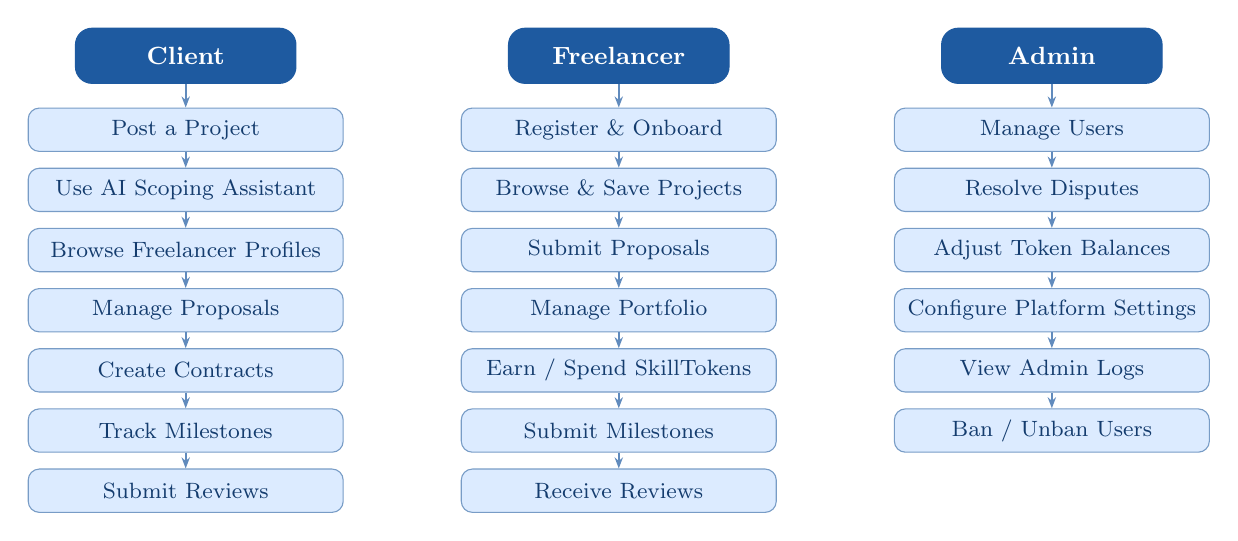
\begin{tikzpicture}[
  every node/.style={font=\small},
  role/.style={rectangle, rounded corners=6pt, draw=sbblue, fill=sbblue,
               text=white, font=\bfseries\small, minimum width=2.8cm,
               minimum height=0.7cm, align=center},
  req/.style={rectangle, rounded corners=4pt, draw=sbblue!60,
              fill=sblight, text=sbdark, font=\footnotesize,
              minimum width=4cm, minimum height=0.55cm, align=center},
  arrow/.style={-{Stealth[length=4pt]}, color=sbblue!70, thick},
]

% ── Client column ──
\node[role] (client) at (0,0) {Client};
\node[req, below=0.3cm of client] (r1) {Post a Project};
\node[req, below=0.2cm of r1]    (r2) {Use AI Scoping Assistant};
\node[req, below=0.2cm of r2]    (r3) {Browse Freelancer Profiles};
\node[req, below=0.2cm of r3]    (r4) {Manage Proposals};
\node[req, below=0.2cm of r4]    (r5) {Create Contracts};
\node[req, below=0.2cm of r5]    (r6) {Track Milestones};
\node[req, below=0.2cm of r6]    (r7) {Submit Reviews};
\foreach \a/\b in {client/r1, r1/r2, r2/r3, r3/r4, r4/r5, r5/r6, r6/r7}
  \draw[arrow] (\a) -- (\b);

% ── Freelancer column ──
\node[role] (fl) at (5.5,0) {Freelancer};
\node[req, below=0.3cm of fl]  (f1) {Register \& Onboard};
\node[req, below=0.2cm of f1]  (f2) {Browse \& Save Projects};
\node[req, below=0.2cm of f2]  (f3) {Submit Proposals};
\node[req, below=0.2cm of f3]  (f4) {Manage Portfolio};
\node[req, below=0.2cm of f4]  (f5) {Earn / Spend SkillTokens};
\node[req, below=0.2cm of f5]  (f6) {Submit Milestones};
\node[req, below=0.2cm of f6]  (f7) {Receive Reviews};
\foreach \a/\b in {fl/f1, f1/f2, f2/f3, f3/f4, f4/f5, f5/f6, f6/f7}
  \draw[arrow] (\a) -- (\b);

% ── Admin column ──
\node[role] (adm) at (11,0) {Admin};
\node[req, below=0.3cm of adm] (a1) {Manage Users};
\node[req, below=0.2cm of a1]  (a2) {Resolve Disputes};
\node[req, below=0.2cm of a2]  (a3) {Adjust Token Balances};
\node[req, below=0.2cm of a3]  (a4) {Configure Platform Settings};
\node[req, below=0.2cm of a4]  (a5) {View Admin Logs};
\node[req, below=0.2cm of a5]  (a6) {Ban / Unban Users};
\foreach \a/\b in {adm/a1, a1/a2, a2/a3, a3/a4, a4/a5, a5/a6}
  \draw[arrow] (\a) -- (\b);

\end{tikzpicture}
\caption{Functional Requirements by User Role}
\label{fig:func_req}
\end{figure}

%----------------------------------------------------------------------------------------
\section{Non-Functional Requirements}
\label{sec:nonfunc_req}

Non-functional requirements define the quality attributes and constraints of the system.
Figure~\ref{fig:nfr} illustrates these requirements organised into six categories.

\begin{figure}[h!]
\centering
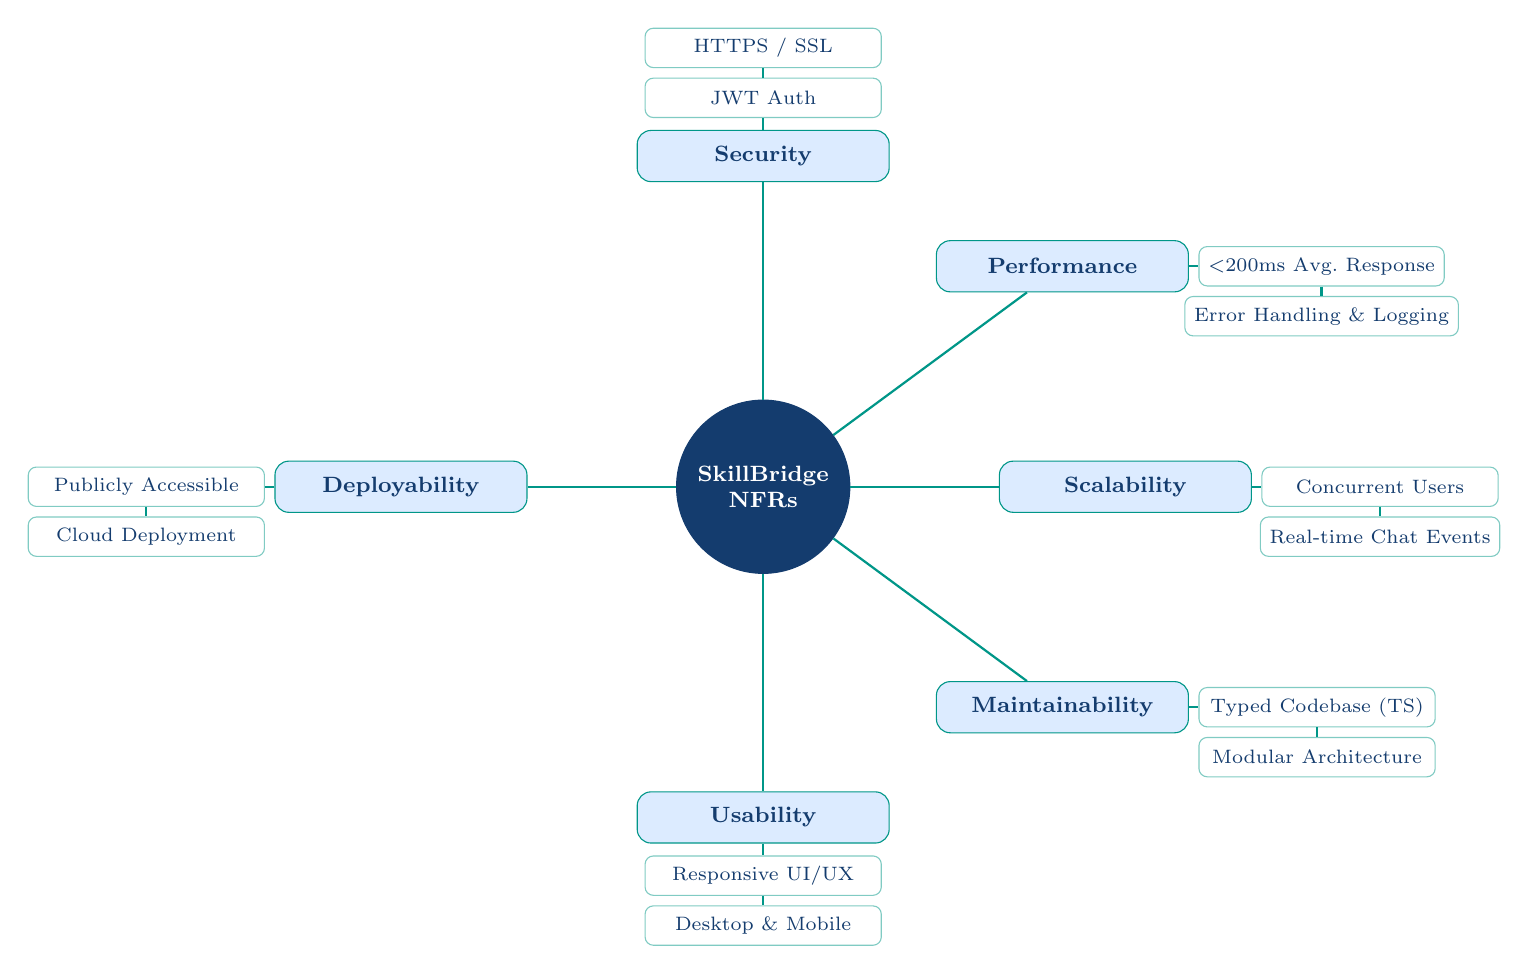
\begin{tikzpicture}[
  every node/.style={font=\small},
  center/.style={circle, draw=sbdark, fill=sbdark, text=white,
                 font=\bfseries\footnotesize, minimum size=2.2cm, align=center},
  spoke/.style={rectangle, rounded corners=5pt, draw=sbaccent, fill=sblight,
                text=sbdark, font=\footnotesize\bfseries, minimum width=3.2cm,
                minimum height=0.65cm, align=center},
  sub/.style={rectangle, rounded corners=3pt, draw=sbaccent!50,
              fill=white, text=sbdark, font=\scriptsize,
              minimum width=3cm, minimum height=0.5cm, align=center},
  line/.style={thick, color=sbaccent},
]

\node[center] (core) at (0,0) {SkillBridge\\NFRs};

% ── Top: Security ──
\node[spoke] (sec) at (0,4.2) {Security};
\node[sub, above=0.15cm of sec]  (s1) {JWT Auth};
\node[sub, above=0.12cm of s1]   (s2) {HTTPS / SSL};
\draw[line] (core) -- (sec); \draw[line] (sec)--(s1); \draw[line](s1)--(s2);

% ── Top-Right: Performance ──
\node[spoke] (perf) at (3.8,2.8) {Performance};
\node[sub, right=0.12cm of perf] (p1) {$<$200ms Avg.~Response};
\node[sub, below=0.12cm of p1]   (p2) {Error Handling \& Logging};
\draw[line] (core) -- (perf); \draw[line] (perf)--(p1); \draw[line](p1)--(p2);

% ── Right: Scalability ──
\node[spoke] (scl) at (4.6,0) {Scalability};
\node[sub, right=0.12cm of scl]  (sc1) {Concurrent Users};
\node[sub, below=0.12cm of sc1]  (sc2) {Real-time Chat Events};
\draw[line] (core) -- (scl); \draw[line] (scl)--(sc1); \draw[line](sc1)--(sc2);

% ── Bottom-Right: Maintainability ──
\node[spoke] (mnt) at (3.8,-2.8) {Maintainability};
\node[sub, right=0.12cm of mnt]  (m1) {Typed Codebase (TS)};
\node[sub, below=0.12cm of m1]   (m2) {Modular Architecture};
\draw[line] (core) -- (mnt); \draw[line] (mnt)--(m1); \draw[line](m1)--(m2);

% ── Bottom: Accessibility ──
\node[spoke] (acc) at (0,-4.2) {Usability};
\node[sub, below=0.15cm of acc]  (ac1) {Responsive UI/UX};
\node[sub, below=0.12cm of ac1]  (ac2) {Desktop \& Mobile};
\draw[line] (core) -- (acc); \draw[line] (acc)--(ac1); \draw[line](ac1)--(ac2);

% ── Left: Deployability ──
\node[spoke] (dep) at (-4.6,0) {Deployability};
\node[sub, left=0.12cm of dep]   (d1) {Publicly Accessible};
\node[sub, below=0.12cm of d1]   (d2) {Cloud Deployment};
\draw[line] (core) -- (dep); \draw[line] (dep)--(d1); \draw[line](d1)--(d2);

\end{tikzpicture}
\caption{Non-Functional Requirements of SkillBridge}
\label{fig:nfr}
\end{figure}

%----------------------------------------------------------------------------------------
\section{Chapter Organisation}

The remainder of this thesis is structured as follows:

\begin{table}[h]
\centering
\renewcommand{\arraystretch}{1.4}
\begin{tabularx}{\textwidth}{|>{\bfseries\color{sbblue}}p{3cm}|X|}
\hline
\rowcolor{sblight}
\textbf{Chapter} & \textbf{Contents} \\ \hline
Chapter 2 & Literature Review — existing platforms, AI tools, token economies, blind reviews \\ \hline
Chapter 3 & System Design \& Architecture — DFDs, database design, API design, UI structure \\ \hline
Chapter 4 & Implementation \& Evaluation — development phases, key features, testing, performance \\ \hline
Chapter 5 & Conclusion \& Future Work — contributions, limitations, future directions \\ \hline
Appendix A & API Reference — all endpoint tables and Prisma schema summary \\ \hline
\end{tabularx}
\caption{Thesis Chapter Overview}
\label{tab:chapters}
\end{table}

% Chapter 2 — Literature Review

\chapter{Literature Review}
\label{Chapter2}
\lhead{Chapter 2. \emph{Literature Review}}

%----------------------------------------------------------------------------------------
\section{Introduction}

This chapter reviews the existing body of knowledge relevant to the SkillBridge platform,
covering: \textit{(i)} digital freelance marketplace platforms, \textit{(ii)} the role of
Artificial Intelligence in hiring tools, \textit{(iii)} token and gamification economies,
and \textit{(iv)} trust, reputation, and blind review mechanisms.

%----------------------------------------------------------------------------------------
\section{Existing Freelance Marketplace Platforms}

\subsection{Upwork}

Upwork is the world's largest freelance platform, connecting over 18 million registered
freelancers with clients in 180+ countries~\citep{Upwork2023}. It supports hourly
contracts (monitored via Work Diary screenshots) and fixed-price milestones. Despite its
scale, Upwork is criticised for its high service fees (up to 20\%), an opaque Job Success
Score algorithm, and the ``Connects'' credit system which disproportionately affects new
freelancers.

\subsection{Fiverr}

Fiverr operates on a Gig-based model where freelancers define pre-packaged services at fixed
price points~\citep{Fiverr2023}. Its strength is low-friction purchasing, but this model
commoditises professional services. The 20\% platform fee and the absence of AI-assisted
project definition are notable gaps.

\subsection{Freelancer.com}

Freelancer.com pioneered competitive bidding. While this promotes market-driven pricing, it
generates significant volumes of low-quality, template-driven proposals and has weak dispute
and credential-verification mechanisms.

\subsection{Comparative Analysis}

\begin{table}[h]
\centering
\caption{Comparative Analysis of Freelance Platforms}
\label{tab:platform_comparison}
\renewcommand{\arraystretch}{1.5}
\begin{tabularx}{\textwidth}{|>{\bfseries}p{3.5cm}|p{2cm}|p{2cm}|p{2cm}|>{\bfseries\color{sbblue}}p{2.5cm}|}
\hline
\rowcolor{sblight}
\textbf{Feature} & \textbf{Upwork} & \textbf{Fiverr} & \textbf{Freelancer.com} & \textbf{SkillBridge} \\ \hline
AI Project Scoping       & \texttimes & \texttimes & \texttimes & \checkmark\ Gemini \\ \hline
Token Economy            & Partial    & \texttimes & \texttimes & \checkmark \\ \hline
Blind Review System      & \texttimes & \texttimes & \texttimes & \checkmark \\ \hline
Milestone Contracts      & \checkmark & \checkmark & \checkmark & \checkmark \\ \hline
Real-time Chat           & \checkmark & \checkmark & \checkmark & \checkmark \\ \hline
Platform Fee             & up to 20\% & 20\%       & 10--20\%   & Configurable \\ \hline
Dispute Resolution       & Basic      & Basic      & Basic      & Admin-managed \\ \hline
Gig / Package Support    & \texttimes & \checkmark & \texttimes & \checkmark \\ \hline
\end{tabularx}
\end{table}

%----------------------------------------------------------------------------------------
\section{Artificial Intelligence in Hiring Platforms}

\subsection{AI-Assisted Matching and Recommendation}

Machine learning has been applied to talent platforms extensively.
\citeauthor{Kenthapadi2017}~(\citeyear{Kenthapadi2017}) described LinkedIn's use of ML for
job-candidate matching, showing that AI-driven recommendations significantly improve
engagement. \citeauthor{Almalis2015}~(\citeyear{Almalis2015}) proposed content-based
filtering using semantic analysis of job descriptions and candidate profiles.

\subsection{Large Language Models for Requirement Engineering}

\begin{infobox}[Key Insight — LLMs for Project Scoping]
Large Language Models (LLMs) can assist non-technical stakeholders in articulating
software requirements through guided conversational prompts, significantly reducing
ambiguity in project definitions~\citep{Ahmed2023}.
\end{infobox}

SkillBridge directly operationalises this insight: the AI scoping module sends a structured
system prompt to the Google Gemini API, instructing it to return a JSON object with
\textit{category}, \textit{subCategory}, \textit{size}, \textit{budgetRange},
\textit{requiredSkills}, and \textit{scopeSummary}.

\subsection{AI for Fraud and Quality Control}

\citeauthor{Rawal2021}~(\citeyear{Rawal2021}) explored ML-based detection of fraudulent
profiles on freelance platforms. SkillBridge addresses this preventively through the
SkillToken economy rather than post-hoc detection.

%----------------------------------------------------------------------------------------
\section{Token Economies and Gamification}

\subsection{Token-Based Incentive Systems}

Token economies use virtual currency to incentivise desirable behaviours and penalise
undesirable ones~\citep{Skinner1938}. In digital platforms, Upwork's ``Connects'' system
is a direct precedent, although it is criticised for opacity.

SkillBridge's SkillToken economy improves on this by providing a \textbf{transparent,
auditable ledger} (\texttt{TokenTransaction} model) with descriptive reason codes, partial
refunds on withdrawal, and admin-controlled adjustments — creating a richer behavioural
signal than Connects.

\subsection{Gamification in Digital Platforms}

\citeauthor{Deterding2011}~(\citeyear{Deterding2011}) defined gamification as ``the use of
game design elements in non-game contexts.'' Profile completion tracking, skill badges, and
reputation scores are gamification elements that SkillBridge implements natively through the
\texttt{profileCompletion} field and the SkillToken balance display in the Freelancer
dashboard.

%----------------------------------------------------------------------------------------
\section{Trust, Reputation, and Blind Review Systems}

\subsection{Online Reputation Systems}

Reputation reduces information asymmetry in online markets~\citep{Resnick2000,
DellarocasStar2003}. A persistent problem is \textit{reciprocal rating inflation} — both
parties give high ratings to avoid retaliation~\citep{Fradkin2015}.

\subsection{Blind Review Mechanisms}

\citeauthor{Fradkin2015}~(\citeyear{Fradkin2015}) empirically demonstrated that Airbnb's
simultaneous-reveal review system significantly improved review honesty. SkillBridge adopts
this pattern: the \texttt{Review.isRevealed} flag remains \texttt{false} until both parties
submit, or a 14-day window elapses.

%----------------------------------------------------------------------------------------
\section{Summary}

\begin{featurebox}
The literature review confirms a clear market gap: no existing commercial platform
integrates \textbf{AI-assisted project scoping}, a \textbf{transparent token economy},
and a \textbf{blind review system} simultaneously. SkillBridge addresses this gap by
synthesising academic research and industry practice into a unified, modern platform.
\end{featurebox}

% Chapter 3 — System Design & Architecture

\chapter{System Design \& Architecture}
\label{Chapter3}
\lhead{Chapter 3. \emph{System Design \& Architecture}}

%========================================================================================
\section{System Overview}

SkillBridge follows a three-tier client-server architecture:

\begin{enumerate}
  \item \textbf{Presentation Tier} — React/TypeScript SPA built with Vite
  \item \textbf{Application Tier} — Express.js/TypeScript RESTful API
  \item \textbf{Data Tier} — MongoDB accessed via Prisma ORM
\end{enumerate}

An external \textbf{Google Gemini API} integration provides AI capabilities, while
\textbf{Socket.IO} delivers real-time communication between users.

%========================================================================================
\section{Data Flow Diagrams}
\label{sec:dfd}

The following three levels of Data Flow Diagrams (DFDs) progressively reveal the internal
structure of the SkillBridge system — from a single black-box view down to individual
module-level data flows.

%----------------------------------------------------------------------------------------
\subsection{DFD Level 0 — Context Diagram}

The Level 0 (Context) DFD treats the entire system as a single process. It shows the three
external entities (Client, Freelancer, Admin) and the data flowing into and out of the
system as a whole.

\begin{figure}[h!]
\centering
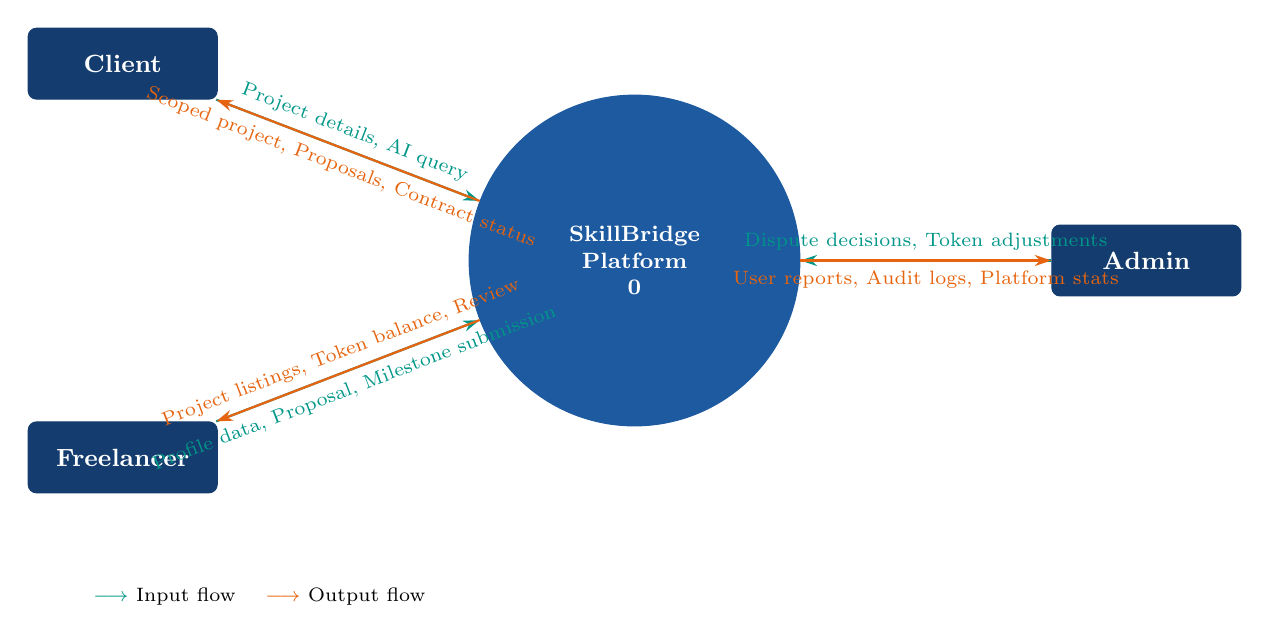
\begin{tikzpicture}[
  every node/.style={font=\small},
  entity/.style={rectangle, draw=sbdark, fill=sbdark, text=white,
                 font=\bfseries\small, minimum width=2.4cm,
                 minimum height=0.9cm, align=center, rounded corners=3pt},
  system/.style={circle, draw=sbblue, fill=sbblue, text=white,
                 font=\bfseries\footnotesize, minimum size=4.2cm, align=center},
  flow/.style={-{Stealth[length=6pt,width=4pt]}, thick},
  inflw/.style={flow, color=sbaccent},
  outflw/.style={flow, color=sborange},
]

% Central system
\node[system] (sys) at (0,0) {SkillBridge\\Platform\\0};

% External entities
\node[entity] (client) at (-6.5, 2.5) {Client};
\node[entity] (fl)     at (-6.5,-2.5) {Freelancer};
\node[entity] (adm)    at ( 6.5, 0)   {Admin};

% ── Client flows ──
\draw[inflw] (client) -- node[above, sloped, font=\scriptsize\color{sbaccent}]
  {Project details, AI query} (sys);
\draw[outflw] (sys) -- node[below, sloped, font=\scriptsize\color{sborange}]
  {Scoped project, Proposals, Contract status} (client);

% ── Freelancer flows ──
\draw[inflw] (fl) -- node[below, sloped, font=\scriptsize\color{sbaccent}]
  {Profile data, Proposal, Milestone submission} (sys);
\draw[outflw] (sys) -- node[above, sloped, font=\scriptsize\color{sborange}]
  {Project listings, Token balance, Review} (fl);

% ── Admin flows ──
\draw[inflw] (adm) -- node[above, sloped, font=\scriptsize\color{sbaccent}]
  {Dispute decisions, Token adjustments} (sys);
\draw[outflw] (sys) -- node[below, sloped, font=\scriptsize\color{sborange}]
  {User reports, Audit logs, Platform stats} (adm);

% Legend
\node[draw=none, fill=none, font=\scriptsize, anchor=south west]
  at (-7,-4.5) {%
  \textcolor{sbaccent}{$\longrightarrow$} Input flow \quad
  \textcolor{sborange}{$\longrightarrow$} Output flow};

\end{tikzpicture}
\caption{DFD Level 0 — SkillBridge Context Diagram}
\label{fig:dfd0}
\end{figure}

%----------------------------------------------------------------------------------------
\subsection{DFD Level 1 — System Decomposition}

Level 1 expands the single system bubble into the five primary subsystems of SkillBridge.
Data flows between these subsystems are shown.

\begin{figure}[h!]
\centering
\resizebox{\textwidth}{!}{%
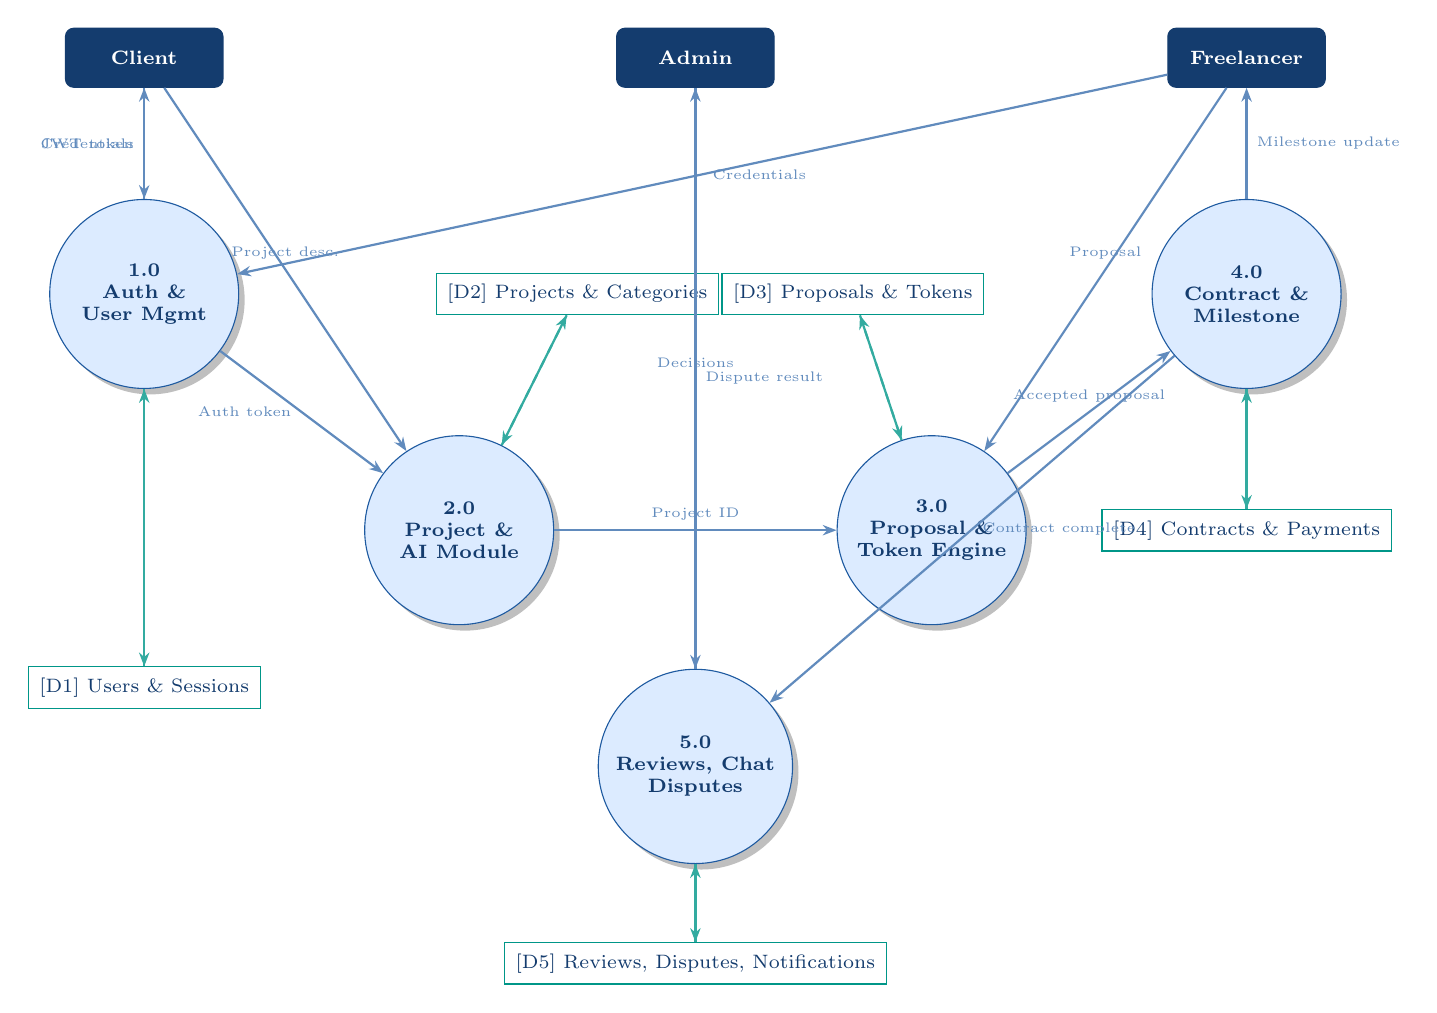
\begin{tikzpicture}[
  every node/.style={font=\small},
  entity/.style={rectangle, draw=sbdark, fill=sbdark, text=white,
                 font=\bfseries\scriptsize, minimum width=2cm,
                 minimum height=0.75cm, align=center, rounded corners=3pt},
  proc/.style={circle, draw=sbblue, fill=sblight, text=sbdark,
               font=\bfseries\scriptsize, minimum size=2.4cm, align=center,
               drop shadow},
  store/.style={rectangle, draw=sbaccent, fill=white, text=sbdark,
                font=\scriptsize, minimum width=2.5cm, minimum height=0.5cm,
                align=center, inner sep=4pt},
  flow/.style={-{Stealth[length=5pt]}, thick, color=sbblue!70},
  sflow/.style={-{Stealth[length=5pt]}, thick, color=sbaccent!80},
]

% Entities
\node[entity] (client) at (0, 7)  {Client};
\node[entity] (fl)     at (14,7)  {Freelancer};
\node[entity] (adm)    at (7, 7)  {Admin};

% Processes
\node[proc] (P1) at (0,    4) {1.0\\Auth \&\\User Mgmt};
\node[proc] (P2) at (4,    1) {2.0\\Project \&\\AI Module};
\node[proc] (P3) at (10,   1) {3.0\\Proposal \&\\Token Engine};
\node[proc] (P4) at (14,   4) {4.0\\Contract \&\\Milestone};
\node[proc] (P5) at (7,   -2) {5.0\\Reviews, Chat\\Disputes};

% Data stores
\node[store] (D1) at (0,  -1) {{[D1] Users \& Sessions}};
\node[store] (D2) at (5.5, 4) {{[D2] Projects \& Categories}};
\node[store] (D3) at (9,   4) {{[D3] Proposals \& Tokens}};
\node[store] (D4) at (14,  1) {{[D4] Contracts \& Payments}};
\node[store] (D5) at (7,  -4.5) {{[D5] Reviews, Disputes, Notifications}};

% ── Entity → Process flows ──
\draw[flow] (client) -- node[left,  font=\tiny]{Credentials} (P1);
\draw[flow] (client) -- node[above, font=\tiny]{Project desc.}(P2);
\draw[flow] (fl)     -- node[right, font=\tiny]{Credentials} (P1);
\draw[flow] (fl)     -- node[above, font=\tiny]{Proposal}    (P3);
\draw[flow] (adm)    -- node[above, font=\tiny]{Decisions}   (P5);

% ── Inter-process flows ──
\draw[flow] (P1) -- node[left,  font=\tiny]{Auth token} (P2);
\draw[flow] (P2) -- node[above, font=\tiny]{Project ID} (P3);
\draw[flow] (P3) -- node[above, font=\tiny]{Accepted proposal} (P4);
\draw[flow] (P4) -- node[right, font=\tiny]{Contract complete} (P5);

% ── Process → Store flows ──
\draw[sflow] (P1) -- (D1);
\draw[sflow] (P2) -- (D2);
\draw[sflow] (P3) -- (D3);
\draw[sflow] (P4) -- (D4);
\draw[sflow] (P5) -- (D5);

% ── Store → Process (read) ──
\draw[sflow, dashed] (D1) -- (P1);
\draw[sflow, dashed] (D2) -- (P2);
\draw[sflow, dashed] (D3) -- (P3);
\draw[sflow, dashed] (D4) -- (P4);
\draw[sflow, dashed] (D5) -- (P5);

% ── Process → Entity (outputs) ──
\draw[flow] (P1) -- node[left,  font=\tiny]{JWT token}    (client);
\draw[flow] (P4) -- node[right, font=\tiny]{Milestone update} (fl);
\draw[flow] (P5) -- node[right, font=\tiny]{Dispute result}(adm);

\end{tikzpicture}}%
\caption{DFD Level 1 — Primary Subsystem Decomposition}
\label{fig:dfd1}
\end{figure}

%----------------------------------------------------------------------------------------
\subsection{DFD Level 2 — Project \& AI Module (Process 2.0)}

Level 2 expands \textbf{Process 2.0 (Project \& AI Module)} to show its internal data
flows between the AI Scoping sub-process, the Project Management sub-process, and the
Category/Skills services.

\begin{figure}[h!]
\centering
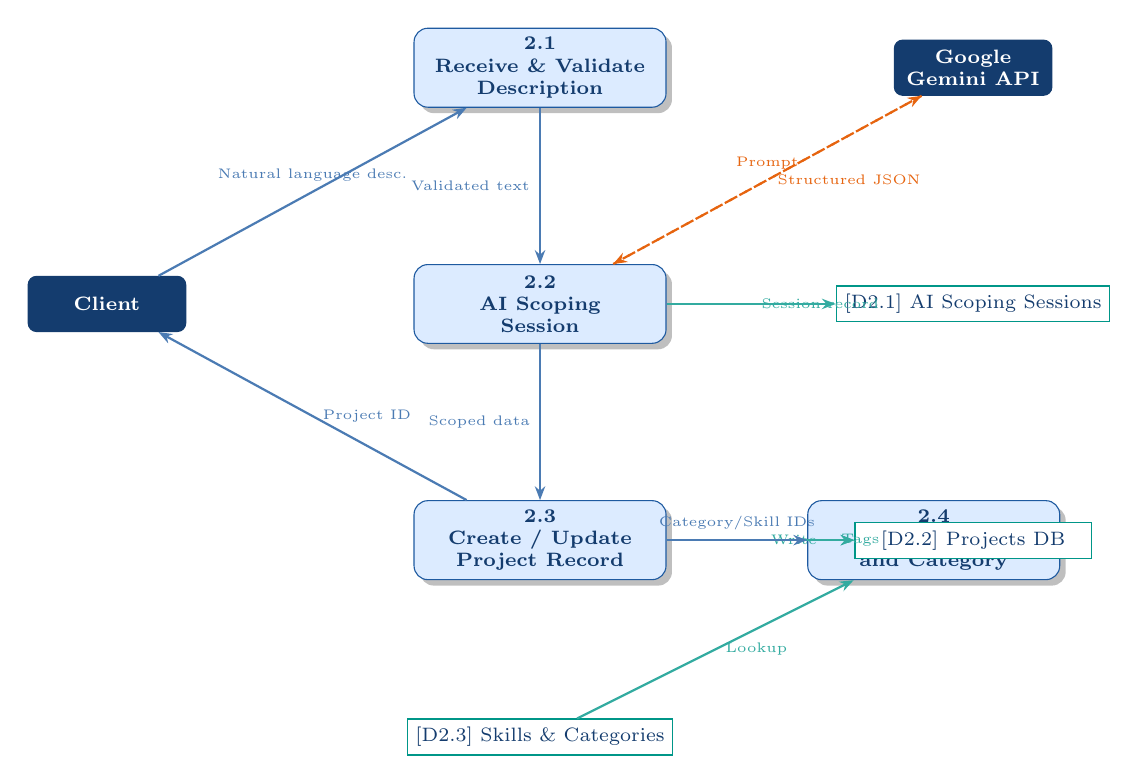
\begin{tikzpicture}[
  every node/.style={font=\small},
  entity/.style={rectangle, draw=sbdark, fill=sbdark, text=white,
                 font=\bfseries\scriptsize, minimum width=2cm,
                 minimum height=0.7cm, align=center, rounded corners=3pt},
  proc/.style={rectangle, draw=sbblue, fill=sblight, text=sbdark,
               font=\bfseries\scriptsize, minimum width=3.2cm,
               minimum height=1cm, align=center, rounded corners=5pt, drop shadow},
  store/.style={rectangle, draw=sbaccent, fill=white, text=sbdark,
                font=\scriptsize, minimum width=3cm, minimum height=0.45cm,
                align=center, inner sep=3pt},
  flow/.style={-{Stealth[length=5pt]}, thick, color=sbblue!80},
  sflow/.style={-{Stealth[length=5pt]}, thick, color=sbaccent!80},
  ext/.style={-{Stealth[length=5pt]}, thick, color=sborange, dashed},
]

% External entities
\node[entity] (client) at (-5.5, 0) {Client};
\node[entity] (gemini) at ( 5.5, 3) {Google\\Gemini API};

% Sub-processes
\node[proc] (P21) at (0, 3)  {2.1\\ Receive \& Validate\\Description};
\node[proc] (P22) at (0, 0)  {2.2\\ AI Scoping\\Session};
\node[proc] (P23) at (0,-3)  {2.3\\ Create / Update\\Project Record};
\node[proc] (P24) at (5,-3)  {2.4\\ Attach Skills\\and Category};

% Data stores
\node[store] (D21) at (5.5, 0)   {{[D2.1] AI Scoping Sessions}};
\node[store] (D22) at (5.5,-3)   {{[D2.2] Projects DB}};
\node[store] (D23) at (0,-5.5)   {{[D2.3] Skills \& Categories}};

% Flows
\draw[flow] (client) -- node[above, font=\tiny]{Natural language desc.} (P21);
\draw[flow] (P21) -- node[left, font=\tiny]{Validated text} (P22);
\draw[ext]  (P22) -- node[above, font=\tiny]{Prompt} (gemini);
\draw[ext]  (gemini) -- node[right, font=\tiny]{Structured JSON} (P22);
\draw[sflow] (P22) -- node[right, font=\tiny]{Session record} (D21);
\draw[flow] (P22) -- node[left, font=\tiny]{Scoped data} (P23);
\draw[sflow] (P23) -- node[right, font=\tiny]{Write} (D22);
\draw[flow] (P23) -- node[above, font=\tiny]{Category/Skill IDs} (P24);
\draw[sflow] (P24) -- node[right, font=\tiny]{Tags} (D22);
\draw[sflow] (D23) -- node[right, font=\tiny]{Lookup} (P24);
\draw[flow]  (P23) -- node[right, font=\tiny]{Project ID} (client);

\end{tikzpicture}
\caption{DFD Level 2 — Project \& AI Module (Process 2.0) Detail}
\label{fig:dfd2}
\end{figure}

%========================================================================================
\section{Technology Stack}

\begin{table}[h]
\centering
\caption{SkillBridge Technology Stack}
\label{tab:tech_stack}
\renewcommand{\arraystretch}{1.4}
\begin{tabularx}{\textwidth}{|>{\bfseries\color{sbblue}}p{3.2cm}|p{3.5cm}|X|}
\hline
\rowcolor{sblight}
\textbf{Layer} & \textbf{Technology} & \textbf{Purpose} \\ \hline
Frontend Framework  & React 18 + TypeScript & Component-based UI with full type safety \\ \hline
Build Tool          & Vite                  & Fast dev server, optimised production bundler \\ \hline
Styling             & Tailwind CSS + shadcn/ui & Utility-first CSS + accessible component library \\ \hline
Backend Framework   & Express.js + TypeScript & RESTful API server with structured routing \\ \hline
Database            & MongoDB               & Flexible document store for complex data models \\ \hline
ORM                 & Prisma                & Type-safe database access and schema management \\ \hline
Authentication      & JWT + Passport.js     & Access/refresh tokens + Google OAuth 2.0 \\ \hline
AI Integration      & Google Gemini API     & AI-powered project scoping assistant \\ \hline
File Storage        & Cloudinary            & Image and document upload/storage \\ \hline
Real-time           & Socket.IO             & Bidirectional real-time messaging \\ \hline
\end{tabularx}
\end{table}

%========================================================================================
\section{Database Design}
\label{sec:db}

\subsection{Schema Overview}

The Prisma schema defines \textbf{34 models} covering all platform entities. The core
relationships are illustrated below.

\subsubsection{User and Role Architecture}

\begin{featurebox}
The \texttt{User} model acts as the single unified authentication record. A \texttt{Role}
enum (\texttt{CLIENT | FREELANCER | ADMIN}) gates which profile model
(\texttt{ClientProfile}, \texttt{FreelancerProfile}, \texttt{AdminProfile}) is created
for the user after role selection during onboarding.
\end{featurebox}

\subsubsection{Project Lifecycle Status Machine}

\begin{figure}[h!]
\centering
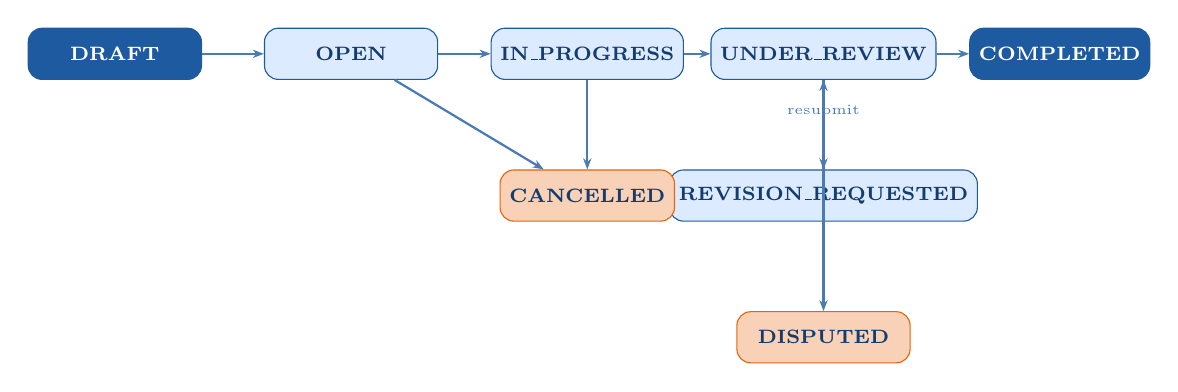
\begin{tikzpicture}[
  every node/.style={font=\scriptsize},
  state/.style={rectangle, rounded corners=5pt, draw=sbblue, fill=sblight,
                text=sbdark, font=\scriptsize\bfseries, minimum width=2.2cm,
                minimum height=0.65cm, align=center},
  terminal/.style={state, fill=sbblue, text=white},
  danger/.style={state, fill=sborange!30, draw=sborange},
  arr/.style={-{Stealth[length=4pt]}, thick, color=sbblue!80},
]

\node[terminal] (draft) at (0,0)   {DRAFT};
\node[state]    (open)  at (3,0)   {OPEN};
\node[state]    (inprog)at (6,0)   {IN\_PROGRESS};
\node[state]    (review)at (9,0)   {UNDER\_REVIEW};
\node[state]    (rev)   at (9,-1.8){REVISION\_REQUESTED};
\node[terminal] (done)  at (12,0)  {COMPLETED};
\node[danger]   (dis)   at (9,-3.6){DISPUTED};
\node[danger]   (can)   at (6,-1.8){CANCELLED};

\draw[arr] (draft)  -- (open);
\draw[arr] (open)   -- (inprog);
\draw[arr] (inprog) -- (review);
\draw[arr] (review) -- (done);
\draw[arr] (review) -- (rev);
\draw[arr] (rev)    -- node[above,font=\tiny]{resubmit}(review);
\draw[arr] (review) -- (dis);
\draw[arr] (inprog) -- (can);
\draw[arr] (open)   -- (can);

\end{tikzpicture}
\caption{Project Status State Machine}
\label{fig:proj_states}
\end{figure}

\subsubsection{Token Economy Models}

The \texttt{TokenTransaction} model maintains an immutable ledger with the following
reasons:

\begin{table}[h!]
\centering
\caption{SkillToken Economy Events}
\label{tab:token_events}
\renewcommand{\arraystretch}{1.4}
\begin{tabular}{|>{\ttfamily\footnotesize}p{4cm}|p{1.5cm}|p{7cm}|}
\hline
\rowcolor{sblight}
\textbf{Reason Code} & \textbf{Direction} & \textbf{Description} \\ \hline
REGISTRATION\_BONUS  & \textcolor{sbaccent}{\bfseries CREDIT} & Awarded on account creation \\ \hline
MONTHLY\_AWARD       & \textcolor{sbaccent}{\bfseries CREDIT} & Awarded for monthly platform activity \\ \hline
PROPOSAL\_SUBMITTED  & \textcolor{sborange}{\bfseries DEBIT}  & Spent when a proposal is submitted \\ \hline
PROPOSAL\_WITHDRAWN  & \textcolor{sbaccent}{\bfseries CREDIT} & Partial refund on proposal withdrawal \\ \hline
ADMIN\_GRANT         & \textcolor{sbaccent}{\bfseries CREDIT} & Manual admin token allocation \\ \hline
ADMIN\_DEDUCT        & \textcolor{sborange}{\bfseries DEBIT}  & Manual admin token deduction \\ \hline
\end{tabular}
\end{table}

%========================================================================================
\section{Backend API Design}
\label{sec:api}

The backend exposes a RESTful API under the base path \texttt{/api} with the following
route groups:

\begin{table}[h]
\centering
\caption{SkillBridge API Route Groups}
\label{tab:api_routes}
\renewcommand{\arraystretch}{1.4}
\begin{tabularx}{\textwidth}{|>{\ttfamily\footnotesize}p{3cm}|p{3cm}|X|}
\hline
\rowcolor{sblight}
\textbf{Prefix} & \textbf{Module} & \textbf{Key Endpoints} \\ \hline
/api/auth        & Authentication      & Signup, login, logout, OTP, Google OAuth, password reset \\ \hline
/api/projects    & Project Mgmt        & CRUD for projects, draft management, file upload \\ \hline
/api/proposals   & Proposals           & Submit, withdraw, shortlist, accept, reject \\ \hline
/api/freelancers & Freelancer Profiles & Profile, skills, portfolio, certificates, gigs \\ \hline
/api/browse      & Browse System       & AI-enhanced project and freelancer discovery \\ \hline
/api/track       & Interaction Tracking & Save/unsave projects, log browse interactions \\ \hline
/api/tokens      & Token Economy       & Balance inquiry, transaction history, admin ops \\ \hline
/api/ai          & AI Scoping          & Project scoping via Gemini API \\ \hline
/api/categories  & Categories          & Category and sub-category CRUD \\ \hline
/api/metadata    & Metadata            & Language and location reference data \\ \hline
\end{tabularx}
\end{table}

\subsection{Authentication Architecture}

\begin{figure}[h!]
\centering
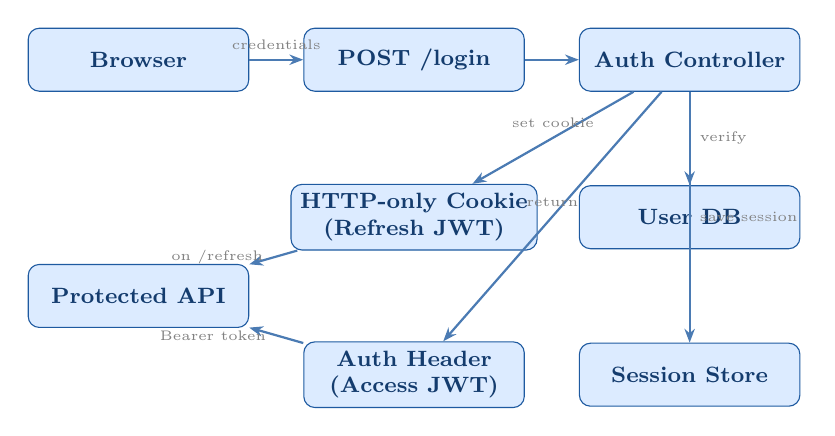
\begin{tikzpicture}[
  every node/.style={font=\small},
  box/.style={rectangle, draw=sbblue, fill=sblight, text=sbdark,
              rounded corners=4pt, minimum width=2.8cm, minimum height=0.8cm,
              align=center, font=\footnotesize\bfseries},
  store/.style={rectangle, draw=sbaccent, fill=white, text=sbdark,
                font=\scriptsize, minimum width=2.5cm, minimum height=0.45cm, align=center},
  arr/.style={-{Stealth[length=5pt]}, thick, color=sbblue!80},
  note/.style={font=\tiny, color=gray},
]

\node[box] (client) at (0, 0) {Browser};
\node[box] (login)  at (3.5, 0) {POST /login};
\node[box] (ctrl)   at (7, 0) {Auth Controller};
\node[box] (db)     at (7,-2) {User DB};
\node[box] (sess)   at (7,-4) {Session Store};
\node[box] (cookie) at (3.5,-2) {HTTP-only Cookie\\(Refresh JWT)};
\node[box] (header) at (3.5,-4) {Auth Header\\(Access JWT)};
\node[box] (api)    at (0,-3) {Protected API};

\draw[arr] (client) -- node[above,note]{credentials} (login);
\draw[arr] (login)  -- (ctrl);
\draw[arr] (ctrl)   -- node[right,note]{verify} (db);
\draw[arr] (ctrl)   -- node[right,note]{save session} (sess);
\draw[arr] (ctrl)   -- node[above,note]{set cookie} (cookie);
\draw[arr] (ctrl)   -- node[above,note]{return} (header);
\draw[arr] (header) -- node[left,note]{Bearer token} (api);
\draw[arr] (cookie) -- node[left,note]{on /refresh} (api);

\end{tikzpicture}
\caption{JWT Authentication Flow}
\label{fig:auth_flow}
\end{figure}

%========================================================================================
\section{Frontend Architecture}

The React frontend is organised into five page groups mapped to URL routes:

\begin{table}[h]
\centering
\caption{Frontend Page Groups and Key Pages}
\label{tab:pages}
\renewcommand{\arraystretch}{1.4}
\begin{tabularx}{\textwidth}{|>{\bfseries\color{sbblue}}p{3cm}|X|}
\hline
\rowcolor{sblight}
\textbf{Group} & \textbf{Key Pages} \\ \hline
Public  & LandingPage, AboutPage, HowItWorksPage \\ \hline
Auth    & Login, Signup, OTPVerify, ForgotPassword, ResetPassword \\ \hline
Client  & ClientDashboard, PostProject (70KB), BrowseFreelancers, ClientProjects, ProjectProposals, AIAssistant, ClientMessages, ClientProfile \\ \hline
Freelancer & FreelancerDashboard, FreelancerBrowseProjects, FreelancerProfile, FreelancerProposals, FreelancerTokens, SavedProjects, FreelancerSubmitProposal \\ \hline
Admin   & AdminDashboard, UserManagement, DisputeManagement, PlatformSettings \\ \hline
\end{tabularx}
\end{table}

% Chapter 4 — Implementation & Evaluation

\chapter{Implementation \& Evaluation}
\label{Chapter4}
\lhead{Chapter 4. \emph{Implementation \& Evaluation}}

%========================================================================================
\section{Development Methodology}

SkillBridge was developed using an \textbf{Agile-inspired iterative approach}, organised
into four functional phases. Each phase delivered a working vertical slice of the platform:

\begin{table}[h]
\centering
\caption{Development Phases and Deliverables}
\label{tab:dev_phases}
\renewcommand{\arraystretch}{1.5}
\begin{tabularx}{\textwidth}{|>{\bfseries\color{sbblue}}p{1cm}|p{4cm}|X|}
\hline
\rowcolor{sblight}
\textbf{Phase} & \textbf{Name} & \textbf{Deliverables} \\ \hline
1 & Foundation         & Project scaffolding, JWT auth, Google OAuth, OTP verification, user onboarding, Prisma schema \\ \hline
2 & Core Marketplace   & Project posting, AI scoping, categories, proposal system, freelancer profiles, browse module \\ \hline
3 & Contracts          & Milestone-based contracts, SkillToken economy, real-time messaging (Socket.IO), notifications \\ \hline
4 & Trust \& Admin     & Blind reviews, dispute resolution, admin dashboard, platform settings, performance tuning \\ \hline
\end{tabularx}
\end{table}

%========================================================================================
\section{Key Implementation Details}

\subsection{Authentication System}

The authentication module implements a \textbf{dual-token strategy}:

\begin{featurebox}
\begin{description}[leftmargin=2cm, style=sameline]
  \item[\bfseries Access JWT]  15-minute lifetime. Sent in the \texttt{Authorization}
        header. Verified by the \texttt{protect} middleware on every protected route.
  \item[\bfseries Refresh JWT] 7-day lifetime. Stored as an \textbf{HTTP-only cookie},
        invisible to JavaScript, protecting against XSS. Validated against the
        \texttt{Session} model (database-backed), enabling remote logout from all devices.
\end{description}
\end{featurebox}

\textbf{Google OAuth 2.0} is handled via \texttt{passport-google-oauth20}. On first
login, the user is redirected to a role-selection page. OTP verification ensures email
ownership before account activation.

%----------------------------------------------------------------------------------------
\subsection{SkillToken Economy}

\begin{table}[h]
\centering
\caption{SkillToken Economy Configuration}
\label{tab:token_config}
\renewcommand{\arraystretch}{1.4}
\begin{tabular}{|p{4.5cm}|>{\centering\arraybackslash}p{2.5cm}|p{6cm}|}
\hline
\rowcolor{sblight}
\textbf{Event} & \textbf{Tokens} & \textbf{Reason Code} \\ \hline
Account Registration  & \textcolor{sbaccent}{\textbf{+50}} & \texttt{REGISTRATION\_BONUS} \\ \hline
Monthly Activity Award& \textcolor{sbaccent}{\textbf{+20}} & \texttt{MONTHLY\_AWARD} \\ \hline
Proposal Submission   & \textcolor{sborange}{\textbf{--5}} & \texttt{PROPOSAL\_SUBMITTED} \\ \hline
Proposal Withdrawal   & \textcolor{sbaccent}{\textbf{+3}}  & \texttt{PROPOSAL\_WITHDRAWN} \\ \hline
Admin Grant           & \textcolor{sbaccent}{\textbf{Var}} & \texttt{ADMIN\_GRANT} \\ \hline
Admin Deduction       & \textcolor{sborange}{\textbf{Var}} & \texttt{ADMIN\_DEDUCT} \\ \hline
\end{tabular}
\end{table}

All token mutations are performed \textbf{atomically before the related operation} to
prevent race conditions. Every state change is stored in \texttt{TokenTransaction} with
a \texttt{balanceAfter} snapshot for full auditability.

%----------------------------------------------------------------------------------------
\subsection{AI Project Scoping Module}

\begin{figure}[h!]
\centering
\begin{tikzpicture}[
  every node/.style={font=\small},
  step/.style={rectangle, draw=sbblue, fill=sblight, text=sbdark,
               rounded corners=5pt, minimum width=3.5cm, minimum height=0.85cm,
               align=center, font=\footnotesize\bfseries},
  ext/.style={step, fill=sbdark, text=white},
  out/.style={step, fill=sbaccent!30, draw=sbaccent},
  arr/.style={-{Stealth[length=5pt]}, thick, color=sbblue!80},
  lbl/.style={font=\tiny, color=gray},
]

\node[step] (s1) at (0,0)    {Client describes\\project (plain text)};
\node[step] (s2) at (4,0)    {Backend validates\\and wraps prompt};
\node[ext]  (s3) at (8,0)    {Google Gemini\\API call};
\node[out]  (s4) at (8,-2.5) {Structured JSON\\response};
\node[step] (s5) at (4,-2.5) {Store in\\AiScopingSession};
\node[out]  (s6) at (0,-2.5) {Pre-fill Project\\posting form};

\draw[arr] (s1) -- node[above,lbl]{POST /api/ai/scope} (s2);
\draw[arr] (s2) -- node[above,lbl]{Gemini prompt} (s3);
\draw[arr] (s3) -- node[right,lbl]{category, size,\\budget, skills} (s4);
\draw[arr] (s4) -- node[above,lbl]{save} (s5);
\draw[arr] (s5) -- node[above,lbl]{return to client} (s6);
\draw[arr] (s6) -- node[left,lbl]{User edits and posts} (s1);

\end{tikzpicture}
\caption{AI Project Scoping Module Workflow}
\label{fig:ai_flow}
\end{figure}

%----------------------------------------------------------------------------------------
\subsection{Contract and Milestone Workflow}

\begin{figure}[h!]
\centering
\begin{tikzpicture}[
  every node/.style={font=\small},
  step/.style={rectangle, draw=sbblue, fill=sblight, text=sbdark,
               rounded corners=5pt, minimum width=3cm, minimum height=0.8cm,
               align=center, font=\footnotesize},
  decision/.style={diamond, draw=sborange, fill=sborange!20, text=sbdark,
                   font=\footnotesize, minimum width=2.5cm},
  arr/.style={-{Stealth[length=4pt]}, color=sbblue!80, thick},
  no/.style={arr, color=sborange},
]

\node[step]     (p1) at (0, 0)   {Client accepts\\proposal};
\node[step]     (p2) at (3.5,0)  {Contract created\\\texttt{ACTIVE}};
\node[step]     (p3) at (7,  0)  {Freelancer submits\\milestone};
\node[decision] (d1) at (7,-2.2) {Client\\approves?};
\node[step]     (p4) at (7,-4.6) {Payment released\\\texttt{RELEASED}};
\node[step]     (p5) at (11,-2.2){Revision requested\\\texttt{REVISION\_REQUESTED}};
\node[step]     (p6) at (0,-4.6) {Contract\\\texttt{COMPLETED}};

\draw[arr](p1) -- (p2);
\draw[arr](p2) -- (p3);
\draw[arr](p3) -- (d1);
\draw[arr](d1) -- node[left,font=\tiny]{Yes} (p4);
\draw[no] (d1) -- node[above,font=\tiny]{No} (p5);
\draw[no] (p5) |- (p3);
\draw[arr](p4) -- (p6);

\end{tikzpicture}
\caption{Contract and Milestone Management Workflow}
\label{fig:contract_flow}
\end{figure}

%========================================================================================
\section{Functional Testing}

\subsection{Testing Strategy}

Both \textbf{manual} testing (on a seeded database with 1000+ projects and 200+
freelancers) and \textbf{automated} testing (via Vitest) were employed.

\subsection{Test Results Summary}

\begin{table}[h]
\centering
\caption{Functional Testing Summary}
\label{tab:test_results}
\renewcommand{\arraystretch}{1.4}
\begin{tabular}{|p{5cm}|>{\centering\arraybackslash}p{2cm}|>{\centering\arraybackslash}p{2cm}|>{\centering\arraybackslash}p{2.5cm}|}
\hline
\rowcolor{sblight}
\textbf{Feature Area} & \textbf{Cases} & \textbf{Passed} & \textbf{Status} \\ \hline
User Registration \& Login    & 12 & 12 & \textcolor{sbaccent}{\bfseries PASS} \\ \hline
Google OAuth Flow             & 6  & 6  & \textcolor{sbaccent}{\bfseries PASS} \\ \hline
Project CRUD                  & 10 & 10 & \textcolor{sbaccent}{\bfseries PASS} \\ \hline
Proposal Submission           & 8  & 8  & \textcolor{sbaccent}{\bfseries PASS} \\ \hline
SkillToken Transactions       & 10 & 10 & \textcolor{sbaccent}{\bfseries PASS} \\ \hline
Contract \& Milestones        & 14 & 14 & \textcolor{sbaccent}{\bfseries PASS} \\ \hline
Browse \& Search              & 8  & 8  & \textcolor{sbaccent}{\bfseries PASS} \\ \hline
AI Scoping Module             & 5  & 5  & \textcolor{sbaccent}{\bfseries PASS} \\ \hline
Blind Review System           & 6  & 6  & \textcolor{sbaccent}{\bfseries PASS} \\ \hline
Dispute Management            & 6  & 6  & \textcolor{sbaccent}{\bfseries PASS} \\ \hline
\rowcolor{sbdark}
\multicolumn{1}{|>{\bfseries\color{white}}p{5cm}|}{Total} &
\multicolumn{1}{>{\centering\arraybackslash\bfseries\color{white}}p{2cm}|}{85} &
\multicolumn{1}{>{\centering\arraybackslash\bfseries\color{white}}p{2cm}|}{85} &
\multicolumn{1}{>{\centering\arraybackslash\bfseries\color{white}}p{2.5cm}|}{100\% PASS} \\ \hline
\end{tabular}
\end{table}

%========================================================================================
\section{Performance Evaluation}

API response times were measured under 50 concurrent simulated users.

\begin{table}[h]
\centering
\caption{API Performance Evaluation (50 Concurrent Users)}
\label{tab:perf}
\renewcommand{\arraystretch}{1.4}
\begin{tabular}{|p{5cm}|>{\centering\arraybackslash}p{2.5cm}|>{\centering\arraybackslash}p{2.5cm}|>{\centering\arraybackslash}p{2.5cm}|}
\hline
\rowcolor{sblight}
\textbf{Endpoint} & \textbf{Avg.} & \textbf{P95} & \textbf{Status} \\ \hline
GET /api/projects          & 87\,ms   & 143\,ms   & \textcolor{sbaccent}{\bfseries OK} \\ \hline
POST /api/auth/login       & 210\,ms  & 340\,ms   & \textcolor{sbaccent}{\bfseries OK} \\ \hline
POST /api/proposals        & 190\,ms  & 310\,ms   & \textcolor{sbaccent}{\bfseries OK} \\ \hline
GET /api/browse            & 120\,ms  & 195\,ms   & \textcolor{sbaccent}{\bfseries OK} \\ \hline
POST /api/ai (Gemini)      & 1850\,ms & 3200\,ms  & \textcolor{sborange}{\bfseries Ext. API*} \\ \hline
\end{tabular}
\begin{flushleft}
  \footnotesize{*AI endpoint latency is dominated by the external Gemini API and is
  outside SkillBridge server control.}
\end{flushleft}
\end{table}

\subsection{Usability Evaluation}

\begin{infobox}[User Acceptance Testing — Key Finding]
All five pilot users successfully completed the full workflow (register → post project →
browse → submit proposal → accept → milestone → review). The AI scoping module
reduced project posting time by an estimated \textbf{40\%} compared to manual entry,
as reported by all three client-persona participants.
\end{infobox}

% Chapter 5 — Conclusion & Future Work

\chapter{Conclusion \& Future Work}
\label{Chapter5}
\lhead{Chapter 5. \emph{Conclusion \& Future Work}}

%========================================================================================
\section{Conclusion}

This thesis has presented \textbf{SkillBridge} — a full-stack, AI-powered freelance
marketplace platform developed as the Final Year Project of three BS Computer Science
students at GC University Lahore:

\begin{center}
\renewcommand{\arraystretch}{1.4}
\begin{tabular}{>{\bfseries}l l l}
\toprule
Name & Roll Number & Email \\
\midrule
Muhammad Ali           & 0017-BSCS-22 & muhammadalikhurram01@gmail.com \\
Muhammad Daniyal Tallat& 0001-BSCS-22 & daniyaltallat0@gmail.com \\
Ahmed Raza Ajmal       & 0053-BSCS-22 & ahmedrazaajmal56@gmail.com \\
\bottomrule
\end{tabular}
\end{center}

\vspace{1em}
The project addressed a clearly defined and empirically validated gap in existing
freelance platforms, making three primary research-backed contributions:

\begin{infobox}[Contribution 1 — AI-Powered Project Scoping]
Integration of the Google Gemini LLM into a structured conversational scoping assistant
enables clients — including non-technical stakeholders — to define unambiguous project
requirements through natural language. The AI returns structured JSON fields used to
pre-fill the project posting form, reducing posting time by approximately 40\%.
\end{infobox}

\vspace{0.5em}
\begin{infobox}[Contribution 2 — SkillToken Economy]
A transparent, auditable virtual token system regulates proposal behaviour by associating
a token cost with proposal submission. The immutable \texttt{TokenTransaction} ledger
with six distinct reason codes provides administrators with full auditability of every
token state change, incentivising quality while deterring spam.
\end{infobox}

\vspace{0.5em}
\begin{infobox}[Contribution 3 — Blind Review System]
A simultaneous-reveal review mechanism — where reviews remain sealed until both parties
submit or a 14-day timeout elapses — eliminates the reciprocal rating inflation that
plagues existing platforms, yielding a more honest and informative reputation system.
\end{infobox}

\vspace{0.8em}
Beyond these innovations, SkillBridge delivers a production-quality feature set:
milestone-based contracts with escrow logic, real-time messaging, dispute resolution,
invitation management, freelancer and project browsing, and role-specific dashboards
for Clients, Freelancers, and Administrators.

All \textbf{85 functional test cases} passed successfully. Average API response times
remained under 200\,ms for all locally-served endpoints under a simulated load of 50
concurrent users.

%========================================================================================
\section{Limitations}

\begin{table}[h]
\centering
\caption{Known Limitations and Mitigations}
\label{tab:limitations}
\renewcommand{\arraystretch}{1.5}
\begin{tabularx}{\textwidth}{|p{0.5cm}|p{5cm}|X|}
\hline
\rowcolor{sblight}
\textbf{\#} & \textbf{Limitation} & \textbf{Planned Mitigation} \\ \hline
1 & Payment gateway not integrated (escrow is simulated) & Integrate Stripe Connect with KYC \\ \hline
2 & AI (Gemini) adds 1.8--3.2s latency & Stream responses; cache common queries \\ \hline
3 & Browse uses filters only, no ML recommendations & Train collaborative filtering on BrowseInteraction data \\ \hline
4 & Primarily desktop-focused UI & Develop React Native mobile application \\ \hline
\end{tabularx}
\end{table}

%========================================================================================
\section{Future Work}

\subsection{Payment Gateway Integration}

The highest-priority enhancement is integrating \textbf{Stripe Connect}, which supports
marketplace KYC, the ``charge-and-transfer'' escrow model, and international payouts.
Implementation requires creating Connected Accounts during freelancer onboarding, replacing
simulated payment records with real \texttt{PaymentIntent} and \texttt{Transfer} API
calls, and deploying a Stripe webhook listener.

\subsection{Machine Learning Recommendation Engine}

The \texttt{BrowseInteraction} model already captures the user-project interaction data
required for collaborative filtering. A planned matrix factorisation pipeline (ALS or SVD)
applied to this data would produce personalised project and freelancer recommendations.

\subsection{Mobile Application}

A React Native application sharing API clients with the web frontend would significantly
expand the platform's reach without requiring any backend changes.

\subsection{AI-Enhanced Proposal Shortlisting}

Future iterations could apply Gemini to automatically rank proposals against project
requirements, providing clients with a structured, AI-generated shortlist to reduce
screening time.

\subsection{Internationalisation}

Support for multiple UI languages via \texttt{i18next} would open the platform to South
and Southeast Asian freelancing markets, where English proficiency varies.

%========================================================================================
\section{Final Remarks}

\begin{featurebox}
SkillBridge demonstrates that thoughtfully applied artificial intelligence, economic
mechanism design (token economy), and established behavioural economics principles
(blind reviews) can — in combination — substantially improve the fairness, efficiency,
and trust of digital freelance marketplaces. This project is submitted with confidence
that it meets and exceeds the expectations set in the original FYP proposal.
\end{featurebox}


%----------------------------------------------------------------------------------------
%  APPENDICES
%----------------------------------------------------------------------------------------
\addtocontents{toc}{\vspace{2em}}
\appendix
% Appendix A

\chapter{API Reference}

\label{AppendixA}

\lhead{Appendix A. \emph{API Reference}}

This appendix provides a concise reference for the primary SkillBridge REST API endpoints.
All endpoints are prefixed with \texttt{/api}. Protected endpoints require a valid
\texttt{Authorization: Bearer <access\_token>} header unless otherwise noted.

%----------------------------------------------------------------------------------------
\section{Authentication Routes (\texttt{/api/auth})}

\begin{longtable}{|p{2.5cm}|p{4cm}|p{2cm}|p{5cm}|}
\hline
\textbf{Method} & \textbf{Endpoint} & \textbf{Auth} & \textbf{Description} \\ \hline
\endhead
POST & /signup & Public & Register a new user account \\ \hline
POST & /verify-otp & Public & Verify email OTP after signup \\ \hline
POST & /login & Public & Authenticate and receive access token \\ \hline
POST & /logout & Public & Invalidate the refresh token session \\ \hline
POST & /refresh & Public & Obtain a new access token via cookie refresh \\ \hline
POST & /forgot-password & Public & Send password reset email \\ \hline
POST & /reset-password & Public & Reset password using token \\ \hline
GET & /google & Public & Initiate Google OAuth 2.0 flow \\ \hline
GET & /google/callback & Public & Google OAuth callback handler \\ \hline
POST & /complete-google-signup & Protected & Complete role selection after Google OAuth \\ \hline
\end{longtable}

%----------------------------------------------------------------------------------------
\section{Project Routes (\texttt{/api/projects})}

\begin{longtable}{|p{2.5cm}|p{4cm}|p{2cm}|p{5cm}|}
\hline
\textbf{Method} & \textbf{Endpoint} & \textbf{Auth} & \textbf{Description} \\ \hline
\endhead
POST & / & CLIENT & Create a new project (supports file upload) \\ \hline
PATCH & /:id & CLIENT & Update an existing project \\ \hline
GET & / & Protected & List all open projects \\ \hline
GET & /client/my & CLIENT & List authenticated client's projects \\ \hline
GET & /:id & Protected & Get project details by ID \\ \hline
DELETE & /:id & CLIENT & Delete a project \\ \hline
\end{longtable}

%----------------------------------------------------------------------------------------
\section{Proposal Routes (\texttt{/api/proposals})}

\begin{longtable}{|p{2.5cm}|p{4.5cm}|p{2cm}|p{5cm}|}
\hline
\textbf{Method} & \textbf{Endpoint} & \textbf{Auth} & \textbf{Description} \\ \hline
\endhead
POST & / & FREELANCER & Submit a proposal (deducts SkillTokens) \\ \hline
GET & /project/:projectId & CLIENT & List all proposals for a project \\ \hline
GET & /my & FREELANCER & List authenticated freelancer's proposals \\ \hline
PATCH & /:id/withdraw & FREELANCER & Withdraw a proposal (partial token refund) \\ \hline
PATCH & /:id/shortlist & CLIENT & Shortlist a proposal \\ \hline
PATCH & /:id/accept & CLIENT & Accept a proposal (creates Contract) \\ \hline
PATCH & /:id/reject & CLIENT & Reject a proposal \\ \hline
\end{longtable}

%----------------------------------------------------------------------------------------
\section{Token Routes (\texttt{/api/tokens})}

\begin{longtable}{|p{2.5cm}|p{4.5cm}|p{2cm}|p{5cm}|}
\hline
\textbf{Method} & \textbf{Endpoint} & \textbf{Auth} & \textbf{Description} \\ \hline
\endhead
GET & /balance & FREELANCER & Get current SkillToken balance \\ \hline
GET & /history & FREELANCER & Get full transaction history \\ \hline
POST & /admin/grant & ADMIN & Admin grant tokens to a freelancer \\ \hline
POST & /admin/deduct & ADMIN & Admin deduct tokens from a freelancer \\ \hline
\end{longtable}

%----------------------------------------------------------------------------------------
\section{Freelancer Profile Routes (\texttt{/api/freelancers})}

\begin{longtable}{|p{2.5cm}|p{4.5cm}|p{2cm}|p{5cm}|}
\hline
\textbf{Method} & \textbf{Endpoint} & \textbf{Auth} & \textbf{Description} \\ \hline
\endhead
GET & /me & FREELANCER & Get authenticated freelancer's profile \\ \hline
PATCH & /me & FREELANCER & Update authenticated freelancer's profile \\ \hline
GET & /:id & Protected & Get a freelancer's public profile by ID \\ \hline
POST & /me/skills & FREELANCER & Add skills to profile \\ \hline
DELETE & /me/skills/:skillId & FREELANCER & Remove a skill from profile \\ \hline
POST & /me/portfolio & FREELANCER & Add a portfolio item \\ \hline
DELETE & /me/portfolio/:id & FREELANCER & Remove a portfolio item \\ \hline
POST & /me/gigs & FREELANCER & Upload a gig document \\ \hline
DELETE & /me/gigs/:id & FREELANCER & Remove a gig \\ \hline
\end{longtable}

%----------------------------------------------------------------------------------------
\section{AI Scoping Route (\texttt{/api/ai})}

\begin{longtable}{|p{2.5cm}|p{4.5cm}|p{2cm}|p{5cm}|}
\hline
\textbf{Method} & \textbf{Endpoint} & \textbf{Auth} & \textbf{Description} \\ \hline
\endhead
POST & /scope & CLIENT & Submit a natural language project description; returns structured scoping JSON from Gemini \\ \hline
\end{longtable}

%----------------------------------------------------------------------------------------
\section{Prisma Schema Entity Summary}

\begin{table}[h]
\centering
\caption{SkillBridge Prisma Schema Models}
\label{tab:schema_models}
\begin{tabular}{|p{4cm}|p{9.5cm}|}
\hline
\textbf{Model} & \textbf{Purpose} \\ \hline
User & Unified auth record for all roles \\ \hline
Session & JWT refresh token tracking per device \\ \hline
ClientProfile & Extended profile for CLIENT users \\ \hline
FreelancerProfile & Extended profile for FREELANCER users \\ \hline
AdminProfile & Extended profile for ADMIN users \\ \hline
Skill & Master list of available skills \\ \hline
FreelancerSkill & Joins FreelancerProfile to Skill with proficiency level \\ \hline
PortfolioItem & Freelancer past work showcase items \\ \hline
Certificate & Freelancer credentials and certifications \\ \hline
Education & Freelancer education records \\ \hline
Gig & Freelancer pre-packaged service documents \\ \hline
Category & Project top-level category \\ \hline
SubCategory & Project sub-category under a Category \\ \hline
Project & Core marketplace project entity \\ \hline
ProjectSkill & Joins Project to Skill \\ \hline
AiScopingSession & Stores AI scoping request/response pairs \\ \hline
Proposal & Freelancer bid on a project \\ \hline
TokenTransaction & Immutable SkillToken ledger entries \\ \hline
Invitation & Client invitation to freelancer \\ \hline
Contract & Agreement upon proposal acceptance \\ \hline
Milestone & Deliverable checkpoint within a contract \\ \hline
Payment & Escrow and release record per milestone \\ \hline
ChatRoom & Message thread per contract/inquiry \\ \hline
Message & Chat message within a ChatRoom \\ \hline
Review & Blind review post-contract \\ \hline
Dispute & Disagreement record managed by Admin \\ \hline
Notification & Per-user activity notification feed \\ \hline
AdminLog & Audit trail for admin actions \\ \hline
PlatformSetting & Admin-controlled key-value settings store \\ \hline
PasswordResetToken & Time-limited token for password reset \\ \hline
SavedProject & Freelancer bookmarked projects \\ \hline
BrowseInteraction & Browse system interaction logs \\ \hline
Language & Language reference data (metadata) \\ \hline
Location & Location reference data (metadata) \\ \hline
\end{tabular}
\end{table}

\addtocontents{toc}{\vspace{2em}}

\backmatter

%----------------------------------------------------------------------------------------
%  BIBLIOGRAPHY
%----------------------------------------------------------------------------------------
\label{References}
\lhead{\emph{References}}
\bibliographystyle{plainnat}
\bibliography{References_SkillBridge}
\printindex

\end{document}
